% exercise sheet with header on every page for math or close subjects
\documentclass[12pt]{article}
\usepackage[utf8]{inputenc} 
\usepackage{latexsym} 
\usepackage{multicol}
\usepackage{fancyhdr}
\usepackage{amsfonts} 
\usepackage{amsmath}
\usepackage{amssymb}
\usepackage{enumerate}
\usepackage{listings}
\usepackage{graphicx}
\usepackage{hyperref}

% Shortcuts for bb, frak and cal letters
\newcommand{\E}{\mathbb{E}}
\newcommand{\V}{\mathbb{V}}
\renewcommand{\P}{\mathbb{P}}
\newcommand{\N}{\mathbb{N}}
\newcommand{\R}{\mathbb{R}}
\newcommand{\C}{\mathbb{C}}
\newcommand{\Z}{\mathbb{Z}}
\newcommand{\Pfrak}{\mathfrak{P}}
\newcommand{\Pfrac}{\mathfrak{P}}
\newcommand{\Bfrac}{\mathfrak{P}}
\newcommand{\Bfrak}{\mathfrak{B}}
\newcommand{\Fcal}{\mathcal{F}}
\newcommand{\Ycal}{\mathcal{Y}}
\newcommand{\Bcal}{\mathcal{B}}
\newcommand{\Acal}{\mathcal{A}}

% formating
\topmargin -1.5cm 
\textheight 24cm
\textwidth 16.0 cm 
\oddsidemargin -0.1cm

% Fancy Header on every Page
\pagestyle{fancy}
\lhead{\textbf{Pattern and Speech Recognition}}
\rhead{Daniel Schäfer (2549458)\\ Christian Bohnenberger (2548364) \\ Dominik Weber (2548553)}
\renewcommand{\headrulewidth}{1.2pt}

\setlength{\headheight}{45pt} 

\begin{document}
\pagenumbering{gobble}

% TODO set the number of the exercise sheet here!
\setcounter{section}{3}

\subsection{Linear Regression}
\begin{enumerate}[a)]

    \item 
        see File \textit{linear-regression.py} (marked in comments)

    \item 
        It is quite obvious that this output can be approximated by a function of degree one.\\
        \begin{center}
            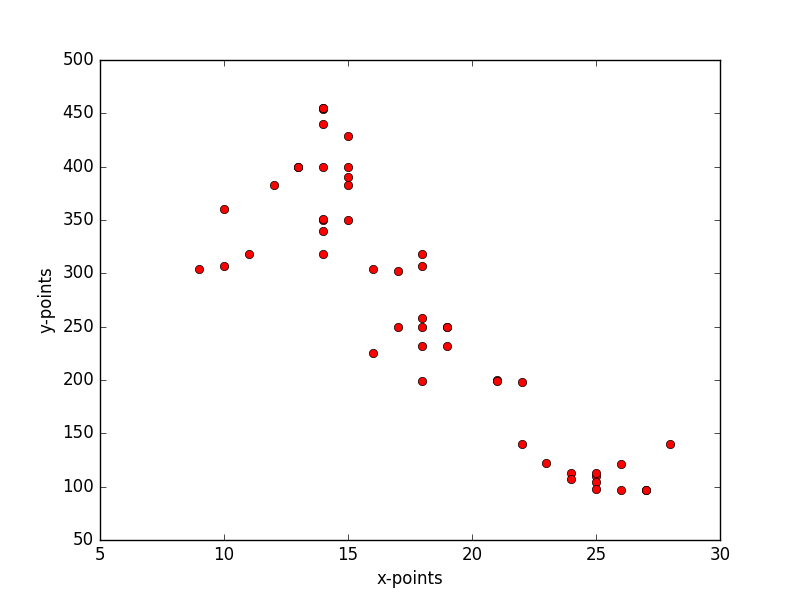
\includegraphics[scale = 0.52]{pictures/train_distr}\\
        \end{center}

    \item 
        Equation for such a model:
        $$ \hat{y} = w*x + b $$

        Gradient descent update rule:
        $$ \nabla_W \text{MSE}_\text{train} = \nabla_W \frac{1}{m} \Vert (X^{(\text{train})} * w - y^{(\text{train})}) \Vert^2_2 $$

    \item 
        % TODO plots and learning rate
        \begin{itemize}
            \item 
                we are initiating random values for W and b and after multiple executions (using learning rate 0.01 and 5000 epochs) we noticed that W seems tend towards $-20$ and b towards $619$. We decided to use these values as our initial values for W and b.

            \item
                After using these initial values and running the same procedure our gradient descent ``resulted'' in $W = -20.49593163$ and $b = 620.40246582$
        \end{itemize}

        using the initial values above and $epochs = 5000$ we are capturing the loss using a specific learningrate:
        \begin{itemize}
            \item
                learningrate = 0.01 $\Rightarrow$ Cost = 1631.553466797
            \item 
                learningrate = 0.02 $\Rightarrow$ Cost = 1691.129394531
            \item
                learningrate = 0.1 $\Rightarrow$ Cost = 2964.26147609
            \item
                learningrate = 0.03 $\Rightarrow$ Cost = 1763.359008789
            \item
                learningrate = 0.001 $\Rightarrow$ Cost = 1540.411987305
            \item
                learningrate = 0.005 $\Rightarrow$ Cost = 1576.098876953
            \item
                learningrate = 0.0001 $\Rightarrow$ Cost = 1539.946899414
        \end{itemize}

    \item 
        % TODO
        TODO insert Task e)

    \item 
        % TODO
        TODO insert Task f)

    \item 
        % TODO
        TODO insert Task g)

    \item 
        % TODO
        TODO insert Task h)

    \item 
        % TODO
        TODO insert Task i)

\end{enumerate}

\subsection{Regularization}


\end{document}
